\documentclass[10pt, oneside, a4paper]{article}
\usepackage{ifpdf}
\usepackage[colorlinks,bookmarksopen,linkcolor=black,pdfauthor={Sharad,Prabhakar,Vikram},urlcolor=blue]{hyperref}
\usepackage{graphicx}

\begin{document}
\begin{center}
\thispagestyle{empty}
\textbf{Sri Jayachamarajendra College of Engineering, Mysore - 570006 \\}
\textbf{\\Department of Computer Science and Engineering}
\vspace{.5in}

\begin{figure}[htb]
\begin{center}
\ifpdf
	
\includegraphics[scale=0.50]{./logo.png}
\else
\fi
\end{center}
\end{figure}
\vspace{.5in}
Software Requirements Specification Document for\\
\textbf{\underline{Telephone Bill Generation Software for Telecom District}} \\
\vspace{.25in}
Nov 2009

\vspace{1in}

THE TEAM \\

\vspace{.1in}
\begin{tabular}{|c|c|c|}
\hline
%% row 1
 Name
& Roll Number  
& USN
\\\hline
%% row 2
Vikram TV 
& 59
& 4JC07CS120
\\\hline
%% row 3
Prabhakar Gouda
& 35
& 4JC07CS070
\\\hline
%% row 4
Sharad D
& 03
& 4JC06CS089
\\\hline
\end{tabular}
\\ **5th Semester 'B' Section
\end{center}
\newpage
\thispagestyle{empty}
\tableofcontents
\newpage
\pagenumbering{arabic}
\section{Objective}

To develop consistent, robust and user-friendly software that generates bills for a ‘telecommunication network provider’ to its customers of a telecom district.

\subsection{Overview}
The software will accept the metered readings and generate bills according to the tariffs set by the provider for various customers.  Bills that are stored in the database can be retrieved and can be displayed.  The software will also provide securities, so that only a specified user can handle the software.
\section{User Requirements:}
\begin{itemize}
\item Customer is able to login to his account to view the bill and the profile.
\item Customer is also able to select the month and view the particular bill and its status (like due date).
\item Clerk from the network provider is able to handle the database and generate bills.
\end{itemize}

\subsection{Users of the System}
\begin{itemize}
\item Customer
\item Administrator
\item Clerk
\end{itemize}

\section{System Requirements}
\begin{itemize}
\item System should maintain the database of customer, call logs and the bill. The database is maintained in a server.
\item The Administrator maintains and monitors the entire system.
\item Clerks generate the bill for the customers.
\item Each customer can have multiple connections and each connection is of  specific tariff. The customer must have maintained a deposit amount.

\item Clerks and customers are able to view  bills based on bill number or customer ID.

\end{itemize}

\section{Functional Requirements}
\begin{itemize}
\item Customer and his telephone number are basic requirements for bill generation. Each customer is provided with a unique customer ID.
\item Customer can have different tariff plans.
\item Call logs are maintained for each customer. Dialled calls are metered.
\item Bill is genereated based on meter reading and tariff at the end of each month. Taxes, Deposits, Debits and Credits are taken care of while billing. Each bill is assigned with a unique bill number.
\item System adds due charges for late payment.
\item Customers can view their bill and profile.
\item An acknowledgement is provided for every payment of the bill.
\end{itemize}
\section{Non-functional Requirements}
\begin{itemize}
\item Every user is provided with a unique login name and password.

\item None of users can modify the call log. Only administrator is able to modify the address of customer if necessary
\item Payment of bill can be done either by cash, cheque or by DD.	
\end{itemize}
\section{Domain Requirements}
\begin{itemize}
\item Bill Generation is for a telecom district.
\item Call logs older than three months are cleared to free up disk space.
\end{itemize}
\section{Optional Features}
\begin{itemize}
\item The system is maintained using web interface and database software.  
\item Only call logs are generated using program to simulate user activities. 
\end{itemize}

\section{User Interface}
\begin{itemize}
\item All users are interfaced using a browser. 
\item Use of Javascript for professional look and feel.

\end{itemize}

\section{Tools to be used}
\begin{itemize}
\item PHP Hypertext Preprocessor
\item Javascript 	
\item Web 2.0
\end{itemize}

\section{Final Deliverable}
\begin{itemize}
\item Archive of Product with Source code.
\item Online Product (for simulation).
\item Online Documentation (for simulation).
\end{itemize}
\begin{thebibliography}B
	BSNL and AIRTEL Telephone Bills.\\
	\href{http://www.data.bsnl.in}{BSNL Portal}\\
	BSNL RTTC, TK Layout, Mysore - for enquiring on Bill Generation.
\end{thebibliography}
\vspace{1in}
\begin{figure}[htb]
\begin{center}
\ifpdf
	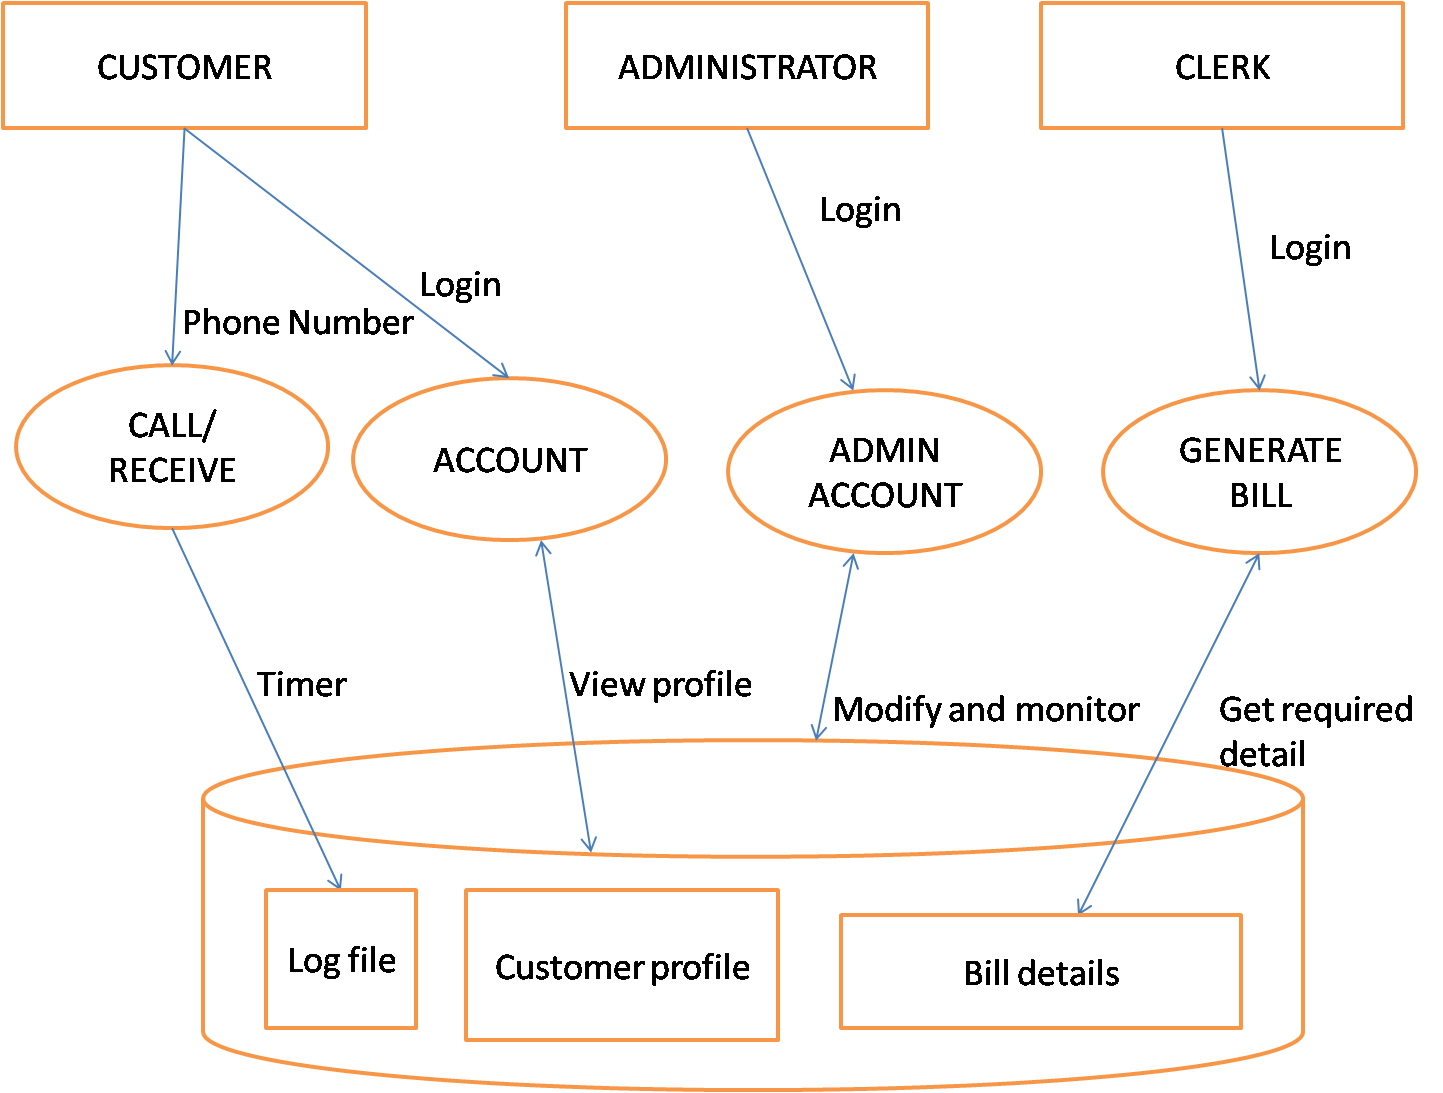
\includegraphics[scale=0.50]{DFD.png}
\else
\fi
\caption{Billing Software Database as viewed from different users.}
\label{DFD}
\end{center}
\end{figure}

\end{document}
